%\documentclass{beamer}
\documentclass[handout]{beamer}

\usepackage{xcolor}
\usepackage{amsmath}

\input ../macros.tex

\beamerdefaultoverlayspecification{<+->}

\definecolor{mathred}{RGB}{200,0,0}
\newcommand{\redmath}[1]{\textcolor{mathred}{#1}}

\mode<presentation>
{
  \usetheme{Montpellier}

  %\setbeamercovered{transparent}
  % or whatever (possibly just delete it)
}

\title{Online Learning and Online Convex Optimization}
\date{}

\begin{document}
\begin{small}
\begin{frame}
  \titlepage
{\bf Chapter 2 in Shai Shalev Shwartz / Online Learning and Online convex Optimization} 
\end{frame}

\begin{frame}
  \frametitle{Outline}
  \tableofcontents[pausesections]
  % You might wish to add the option [pausesections]
\end{frame}

\section{Online Convex Optimization}
\begin{frame}{Online Convex Optimization (OCO)}
\begin{block}{Algorithm}
\textbf{Input:} A convex set \( \textcolor{red}{S} \)

\textbf{For} \( \textcolor{red}{t = 1,2,\dots} \)
\begin{itemize}
    \item Predict a vector \( \textcolor{red}{w_t \in S} \)
    \item Receive a convex loss function \( \textcolor{red}{f_t: S \to \mathbb{R}} \)
    \item Suffer loss \( \textcolor{red}{f_t(w_t)} \)
\end{itemize}
\end{block}
\end{frame}

\begin{frame}{Regret Definition}
    \textbf{Regret of the Algorithm:}
    \begin{equation}
        \textcolor{red}{\text{Regret}_T(u) = \sum_{t=1}^{T} f_t(w_t) - \sum_{t=1}^{T} f_t(u).}
    \end{equation}
    \textbf{Regret relative to a set of vectors \( U \):}
    \begin{equation}
        \textcolor{red}{\text{Regret}_T(U) = \max_{u \in U} \text{Regret}_T(u).}
    \end{equation}
\end{frame}


\newcommand{\mathred}[1]{\textcolor{red}{#1}} % New command for red math
\section{Follow The Leader}
\begin{frame}{Follow-the-Leader Algorithm}
\begin{block}{FTL Strategy}
At round $\mathred{t}$, select:
\[
\mathred{w_t = \operatorname{argmin}_{w \in S} \sum_{i=1}^{t-1} f_i(w)}
\]
\end{block}

\begin{itemize}
\item Natural approach: Choose best performer on past data
\item Simple but can be unstable
\item Requires solving optimization problem each round
\end{itemize}
\end{frame}

\begin{frame}{FTL Regret Analysis}
\begin{theorem}[Lemma 2.1]
  For any $\mathred{u \in S}$:
  \R{\[
    \text{Regret}_T(\mathbf{u}) = \sum_{t=1}^{T} \left(f_t(\mathbf{w}_t) - f_t(\mathbf{u})\right) \leq \sum_{t=1}^{T} \left(f_t(\mathbf{w}_t) - f_t(\mathbf{w}_{t+1})\right).
  \]}
\end{theorem}
{\bf proof} \\
{\bf Step 1:} Equivalent to
\R{$$
\sum_{t=1}^{T} f_t(\mathbf{w}_{t+1}) \leq \sum_{t=1}^{T} f_t(\mathbf{u})
$$}
\end{frame}

\begin{frame}

{\bf Step 2:} By induction on $\mathred{T}$:
\begin{itemize}
\item \textcolor{red}{Base case:} $\mathred{T=1}$ trivial as $\mathred{f_1(w_1) - f_1(u) \leq 0}$

\item \textcolor{red}{Inductive step:} Assume holds for $\mathred{T-1}$, then
\begin{align*}
\mathred{\sum_{t=1}^T} &\mathred{[f_t(w_t) - f_t(u)]} \\
&\mathred{= \underbrace{\sum_{t=1}^{T-1} [f_t(w_t) - f_t(u)]}_{\leq \sum_{t=1}^{T-1} [f_t(w_t) - f_t(w_{t+1})]} + [f_T(w_T) - f_T(u)]} \\
&\mathred{\leq \sum_{t=1}^T [f_t(w_t) - f_t(w_{t+1})]}
\end{align*}
using $\mathred{w_{T+1} = \operatorname{argmin}_w \sum_{t=1}^T f_t(w)}$
\end{itemize}
\end{frame}

\subsection{Quadratic Optimization}
\begin{frame}{FTL for Quadratic Optimization}
For $\mathred{f_t(w) = \frac{1}{2}\|w - z_t\|_2^2}$:
\begin{itemize}
\item FTL update: $\mathred{w_t = \frac{1}{t-1}\sum_{i=1}^{t-1} z_i}$
\item Regret bound: $\mathred{O(\log T)}$
\end{itemize}
\begin{proof}[Regret Calculation for quadratic optimization]
\begin{align*}
\mathred{\text{Regret}_T(u)} &\mathred{\leq \sum_{t=1}^T \frac{1}{t} \|w_t - z_t\|^2} \\
&\mathred{\leq \sum_{t=1}^T \frac{(2L)^2}{t} = 4L^2(\log T + 1)}
\end{align*}
where $\mathred{L = \max_t \|z_t\|}$
\end{proof}
\end{frame}

\subsection{Failure of Follow the Leader}

\begin{frame}{Failure of follow the leader}
$\mathred{f_t(w) = w \cdot z}$:
\begin{itemize}
\item
  $$z_t= \begin{cases}
           -0.5 & \text{ if } t=1\\
           1 & \text{ if } t \text{ is even} \\
           -1 & \text{ if } t>1 \mbox{ and } t \text{ is odd}
         \end{cases}
         $$
         \item $w_t=-1,1,-1,1,\ldots$
  \item Cumulative loss is $T$.
  \item Cumulative loss of $0$ is $0$
  \item Regret is $T$.
  \item {\bf Reason:} prediction is unstable
  \item We need to regularize.
    \item \R{$R(W)$} penalizes vectors which are large.
  \end{itemize}
\end{frame}

\section{Follow The Regularized Leader}
\begin{frame}{Follow-the-Regularized-Leader (FTRL)}
        \begin{equation*}
            \forall t, \quad \mathbf{w}_t = \arg\min_{\mathbf{w} \in S} \sum_{i=1}^{t-1} f_i(\mathbf{w}) + R(\mathbf{w})
        \end{equation*}
\begin{itemize}
  \item For bad case above: $w_t=0,0,0,0,\ldots$
  \item Each step requires solving a minimization problem.
    \end{itemize}
\end{frame}


\begin{frame}{Lemma 2.3: Follow-the-Regularized-Leader}
    \textbf{Lemma 2.3.} Let $\mathbf{w}_1, \mathbf{w}_2, \dots$ be the sequence of vectors produced by FoReL. Then, for all $\mathbf{u} \in S$ we have:
\R{    \begin{equation*}
        \sum_{t=1}^{T} (f_t(\mathbf{w}_t) - f_t(\mathbf{u})) \leq R(\mathbf{u}) - R(\mathbf{w}_1) + \sum_{t=1}^{T} (f_t(\mathbf{w}_t) - f_t(\mathbf{w}_{t+1})).
    \end{equation*}}
\end{frame}


\begin{frame}{Proof of Lemma 2.3}
    \textit{Proof.} Observe that running FoReL on \R{$f_1, \dots, f_T$} is equivalent to running FTL on \R{$f_0, f_1, \dots, f_T$} where $f_0 = R$. Using Lemma 2.1, we obtain:
\R{    \begin{equation*}
        \sum_{t=0}^{T} (f_t(\mathbf{w}_t) - f_t(\mathbf{u})) \leq \sum_{t=0}^{T} (f_t(\mathbf{w}_t) - f_t(\mathbf{w}_{t+1})).
    \end{equation*}}
    Rearranging the above and using $f_0 = R$, we conclude our proof. \hfill $\square$
  \end{frame}

  \subsection{FTRL for linear functions}
  \begin{frame}{FTRL Regret Bound for linear functions}
    \B{\bf For linear} $\mathred{f_t(w) = \langle w,z_t\rangle}$ and $\mathred{R(w) = \frac{1}{2\eta}\|w\|_2^2}$\\
    \B{\bf Update rule} \R{$w_{t+1}=w_t - \eta z_t$}
    Then, for all \(\mathbf{u}\) we have
    \begin{equation*}
        \textcolor{red}{\text{Regret}_T(\mathbf{u}) \leq \frac{1}{2\eta} \|\mathbf{u}\|_2^2 + \eta \sum_{t=1}^{T} \|\mathbf{z}_t\|_2^2.}
    \end{equation*}
\end{frame}

\begin{frame}{Choice of \(\eta\) and Final Bound for linear functions}
    \textbf{Tunings:}
    \begin{itemize}
        \item Define the set \(\textcolor{red}{U = \{\mathbf{u} : \|\mathbf{u}\| \leq B\}}\).
        \item Assume that
        \[
        \textcolor{red}{\frac{1}{T} \sum_{t=1}^{T} \|\mathbf{z}_t\|_2^2 \leq L^2.}
        \]
        \item Set \(\textcolor{red}{\eta = \frac{B}{L\sqrt{2T}}}\).
    \end{itemize}

    \textbf{Conclusion:}
    \begin{equation*}
        \textcolor{red}{\text{Regret}_T(U) \leq B L \sqrt{2T}.}
    \end{equation*}
\end{frame}

\subsection{Online Gradient Descent}
\begin{frame}{From linear functions to Online Gradient Descent}
\begin{example}[OGD from FTRL]
  Consider the OCO setup where the functions $f_1,f_2,\ldots$ are differentiable.\\
  Let $\eta$ be the learning rate.
\[
  \mathred{w_{t+1} = w_t - \eta z_t,\;\;
    z_t = \nabla f_t(w_t)}
\]
Identical to FTRL with regularization: $\mathred{R(w) = \frac{1}{2\eta}\|w\|_2^2}$
\end{example}


{\bf Regret bound on OGD:} From FTRL theorem:
\begin{align*}
\mathred{\text{Regret}} &\mathred{\leq \frac{\|u\|^2}{2\eta} + \eta \sum_{t=1}^T \|z_t\|^2} \\
&\mathred{\leq \frac{B^2}{2\eta} + \eta T L^2}
\end{align*}
\end{frame}

\begin{frame}{Regret Bound for OGD}
  If we further assume that each \(\textcolor{red}{f_t}\) is \(\textcolor{red}{L_t}\)-Lipschitz with respect to \(\textcolor{red}{\|\cdot\|_2}\),
  and let \(\textcolor{red}{L}\) be such that 
  \[
    \textcolor{red}{\frac{1}{T} \sum_{t=1}^{T} L_t^2 \leq L^2.}
  \]
  Then, for all \(\textcolor{red}{\mathbf{u}}\), the regret of OGD satisfies
  \begin{equation*}
    \textcolor{red}{\text{Regret}_T(\mathbf{u}) \leq \frac{1}{2\eta} \|\mathbf{u}\|_2^2 + \eta T L^2.}
  \end{equation*}
\end{frame}

\begin{frame}{Bounding the norm of \R{$\mathbf{u}$}}
    In particular, if \(\textcolor{red}{U = \{\mathbf{u} : \|\mathbf{u}\|_2 \leq B\}}\) and 
    \(\textcolor{red}{\eta = \frac{B}{L\sqrt{2T}}}\) then

    \begin{equation*}
        \textcolor{red}{\text{Regret}_T(U) \leq B L \sqrt{2T}.}
    \end{equation*}
\end{frame}

\subsection{Doubling Trick}
\begin{frame}{Practical Considerations}
\begin{block}{Doubling Trick}
\begin{itemize}
\item Removes need to know time horizon $\mathred{T}$
\item Divide time into epochs $\mathred{2^m,2^{m+1}-1}$
\item Regret increases by constant factor:
\[
\mathred{\sum_{m=0}^{\log T} \sqrt{2^m} = O(\sqrt{T})}
\]
\end{itemize}
\end{block}

\begin{example}[Optimal $\mathred{\eta}$]
Setting $\mathred{\eta = \frac{B}{L}\sqrt{\frac{2}{T}}}$ gives:
\[
\mathred{BL\sqrt{2T}}
\]
\end{example}
\end{frame}

\subsection{Strong Convexity}
\begin{frame}{Definition 2.4: Strong Convexity}
    \begin{block}{Strong Convexity}
        A function \( f: S \to \mathbb{R} \) is \(\sigma\)-strongly convex over \( S \) with respect to a norm \( \|\cdot\| \) if for any \( \mathbf{w} \in S \) we have:
        \begin{equation*}
            \forall \mathbf{z} \in \partial f(\mathbf{w}), \quad \forall \mathbf{u} \in S, \quad 
            f(\mathbf{u}) \geq f(\mathbf{w}) + \langle \mathbf{z}, \mathbf{u} - \mathbf{w} \rangle + \frac{\sigma}{2} \|\mathbf{u} - \mathbf{w}\|^2.
        \end{equation*}
    \end{block}
\end{frame}

\begin{frame}{Lemma 2.8: Strong Convexity implication}
    \begin{block}{Lemma 2.8}
        Let \( S \) be a nonempty convex set. Let \( f: S \to \mathbb{R} \) be a \( \sigma \)-strongly convex function over \( S \) with respect to a norm \( \|\cdot\| \). Let:
        \[
        \mathbf{w} = \arg\min_{\mathbf{v} \in S} f(\mathbf{v}).
        \]
        Then, for all \( \mathbf{u} \in S \), we have:
        \begin{equation*}
            f(\mathbf{u}) - f(\mathbf{w}) \geq \frac{\sigma}{2} \|\mathbf{u} - \mathbf{w}\|^2.
          \end{equation*}
    \end{block}
\end{frame}

\begin{frame}{Strong Convexity Condition}
    If \( R \) is twice differentiable, then it is easy to verify that a sufficient condition for strong convexity of \( R \) is that for all \( \redmath{\mathbf{w}, \mathbf{x}} \),
    \[
    \langle \redmath{\nabla^2 R(\mathbf{w}) \mathbf{x}}, \redmath{\mathbf{x}} \rangle \geq \redmath{\sigma \|\mathbf{x}\|^2},
    \]
    where \( \redmath{\nabla^2 R(\mathbf{w})} \) is the Hessian matrix of \( R \) at \( \redmath{\mathbf{w}} \), namely, the matrix of second-order partial derivatives of \( R \) at \( \redmath{\mathbf{w}} \) [39, Lemma 14].
\end{frame}


\begin{frame}
    \frametitle{Example 2.4: Euclidean Regularization}
    The function 
    \[
    \textcolor{red}{R(\mathbf{w}) = \frac{1}{2} \|\mathbf{w}\|_2^2}
    \]
    is 1-strongly-convex with respect to the $\ell_2$ norm over $\mathbb{R}^d$. To see this, simply note that the Hessian of $R$ at any $\mathbf{w}$ is the identity matrix.
\end{frame}

\begin{frame}
    \frametitle{Example 2.5: Entropic Regularization}
    The function 
    \[
    \textcolor{red}{R(\mathbf{w}) = \sum_{i=1}^{d} w[i] \log(w[i])}
    \]
    is \textcolor{red}{$\frac{1}{B}$}-strongly-convex with respect to the $\ell_1$ norm over the set 
    \[
    \textcolor{red}{S = \{\mathbf{w} \in \mathbb{R}^d : \mathbf{w} > 0 \wedge \|\mathbf{w}\|_1 \leq B\}}.
    \]
    In particular, $R$ is 1-strongly-convex over the probability simplex, which is the set of positive vectors whose elements sum to 1.
\end{frame}

\begin{frame}
    \frametitle{Proof of strong convexity for Entropic Regularization}
    $\frac{\partial^2}{\partial w[i]^2} w[i] \log w[i] = \frac{1}{w[i]}$ 
    \[
    \textcolor{red}{\langle \nabla^2 R(\mathbf{w})\mathbf{x},\mathbf{x} \rangle = \sum_i \frac{x[i]^2}{w[i]}}
    \]
    \[
    \textcolor{red}{= \frac{1}{\|\mathbf{w}\|_1} \left(\sum_i w[i] \right) \left(\sum_i \frac{x[i]^2}{w[i]} \right)}
    \]
    \[
    \textcolor{red}{\geq \frac{1}{\|\mathbf{w}\|_1} \left(\sum_i \sqrt{w[i]} \frac{x[i]}{\sqrt{w[i]}} \right)^2 = \frac{\|\mathbf{x}\|_1^2}{\|\mathbf{w}\|_1},}
    \]
    where the inequality follows from Cauchy–Schwarz inequality.
\end{frame}

\subsection{General Theorem regarding FTRL with Strong Convexity}
\begin{frame}
    \frametitle{Single Step of FTRL with Strong Convexity}
    Let 
    \[
    \textcolor{red}{R : S \to \mathbb{R}}
    \]
    be a \textcolor{red}{$\sigma$}-strongly-convex function over $S$ with respect to a norm \textcolor{red}{$\|\cdot\|$}. Let \textcolor{red}{$\mathbf{w}_1, \mathbf{w}_2, \dots$} be the predictions of the FoReL algorithm. Then, for all $t$, if \textcolor{red}{$f_t$} is \textcolor{red}{$L_t$}-Lipschitz with respect to \textcolor{red}{$\|\cdot\|$}, then:
    \[
    \textcolor{red}{f_t(\mathbf{w}_t) - f_t(\mathbf{w}_{t+1}) \leq L_t \|\mathbf{w}_t - \mathbf{w}_{t+1}\| \leq \frac{L_t^2}{\sigma}.}
    \]
\end{frame}

\begin{frame}
    \frametitle{Proof (Single Step of FTRL with Strong Convexity)}
    For all $t$ let 
    \[
    \textcolor{red}{F_t(\mathbf{w}) = \sum_{i=1}^{t-1} f_i(\mathbf{w}) + R(\mathbf{w})}
    \]
    and note that the FoReL rule is 
    \[
    \textcolor{red}{\mathbf{w}_t = \arg\min_{\mathbf{w} \in S} F_t(\mathbf{w})}.
    \]
    Note also that $F_t$ is \textcolor{red}{$\sigma$}-strongly-convex since the addition of a convex function to a strongly convex function keeps the strong convexity property. Therefore, Lemma 2.8 implies that:
    \[
    \textcolor{red}{F_t(\mathbf{w}_{t+1}) \geq F_t(\mathbf{w}_t) + \frac{\sigma}{2} \|\mathbf{w}_t - \mathbf{w}_{t+1}\|^2.}
    \]
\end{frame}

\begin{frame}
    \frametitle{Continuing the Proof (Single Step of FTRL with Strong Convexity)}
    Repeating the same argument for $F_{t+1}$ and its minimizer $\mathbf{w}_{t+1}$, we get:
    \[
    \textcolor{red}{F_{t+1}(\mathbf{w}_t) \geq F_{t+1}(\mathbf{w}_{t+1}) + \frac{\sigma}{2} \|\mathbf{w}_t - \mathbf{w}_{t+1}\|^2.}
    \]
    Taking the difference between the last two inequalities and rearranging, we obtain:
    \[
    \textcolor{red}{\sigma \|\mathbf{w}_t - \mathbf{w}_{t+1}\|^2 \leq f_t(\mathbf{w}_t) - f_t(\mathbf{w}_{t+1}).} \quad (2.7)
    \]
\end{frame}

\begin{frame}
    \frametitle{Final Steps (Single Step of FTRL with Strong Convexity)}
    Next, using the Lipschitzness of $f_t$, we get that:
    \[
    \textcolor{red}{f_t(\mathbf{w}_t) - f_t(\mathbf{w}_{t+1}) \leq L_t \|\mathbf{w}_t - \mathbf{w}_{t+1}\|.}
    \]
    Combining with Equation (2.7) and rearranging, we get:
    \[
    \textcolor{red}{\|\mathbf{w}_t - \mathbf{w}_{t+1}\| \leq L / \sigma.}
    \]
    Together with the above, we conclude our proof. \hfill \(\blacksquare\)
\end{frame}

\begin{frame}
    \frametitle{Main theorem regarding $\sigma$-strongly convex regularization functions}
    Let 
    \textcolor{red}{$f_1, \dots, f_T$} 
    be a sequence of convex functions such that 
    \textcolor{red}{$f_t$} 
    is 
    \textcolor{red}{$L_t$}-Lipschitz 
    with respect to some norm \textcolor{red}{$\|\cdot\|$}. Let 
    \textcolor{red}{$L$} 
    be such that 
    \[
    \textcolor{red}{\frac{1}{T} \sum_{t=1}^{T} L_t^2 \leq L^2.}
    \]
    Assume that FoReL is run on the sequence with a regularization function which is 
    \textcolor{red}{$\sigma$}-strongly-convex 
    with respect to the same norm. Then, for all 
    \textcolor{red}{$\mathbf{u} \in S$},
    \[
    \textcolor{red}{\operatorname{Regret}_T(\mathbf{u}) \leq R(\mathbf{u}) - \min_{\mathbf{v} \in S} R(\mathbf{v}) + \frac{T L^2}{\sigma}.}
    \]
\end{frame}

\begin{frame}
    \frametitle{Corollary for $l_2$ regularization}
    Let 
    \textcolor{red}{$f_1, \dots, f_T$} 
    be a sequence of convex functions such that 
    \textcolor{red}{$f_t$} 
    is 
    \textcolor{red}{$L_t$}-Lipschitz 
    with respect to \textcolor{red}{$\|\cdot\|_2$}. Let 
    \textcolor{red}{$L$} 
    be such that 
    \[
    \textcolor{red}{\frac{1}{T} \sum_{t=1}^{T} L_t^2 \leq L^2.}
    \]
    Assume that FoReL is run on the sequence with the regularization function 
    \[
    \textcolor{red}{R(\mathbf{w}) = \frac{1}{2\eta} \|\mathbf{w}\|_2^2.}
    \]
    Then, for all \textcolor{red}{$\mathbf{u}$},
    \[
    \textcolor{red}{\operatorname{Regret}_T(\mathbf{u}) \leq \frac{1}{2\eta} \|\mathbf{u}\|_2^2 + \eta T L^2.}
    \]
\end{frame}

\subsection{Applications to expert advice}

\begin{frame}{Applications to expert advice}
  \begin{itemize}
    \item Distribution \R{$w_t$}
    \item Action Losses: \R{$x_t \in [0,1]^d$}
    \item Algorithm Loss: \R{$\langle x_t, w_t \rangle$}
    \item We want to bound regret.
    \item we will compare $l_2$ regularization with Entropic
      Regularization.
  \end{itemize}
\end{frame}


\begin{frame}
    \frametitle{Experts using \R{$l_2$} regularization (1)}
    \textcolor{red}{$S$} 
    be a convex set and consider running FoReL with the regularization function:
    \[
    \textcolor{red}{R(\mathbf{w}) = 
    \begin{cases} 
    \frac{1}{2\eta} \|\mathbf{w}\|_2^2 & \text{if } \mathbf{w} \in S \\ 
    \infty & \text{if } \mathbf{w} \notin S 
    \end{cases}}
    \]
    Where $S$ us the $d$ dimensional simplex.

    Then, for all 
    \textcolor{red}{$\mathbf{u} \in S$},
    \[
    \textcolor{red}{\operatorname{Regret}_T(\mathbf{u}) \leq \frac{1}{2\eta} \|\mathbf{u}\|_2^2 + \eta T L^2.}
    \]
\end{frame}

\begin{frame}
    \frametitle{Experts using \R{$l_2$} regularization (2)}
    If 
    \[
    \textcolor{red}{B \geq \max_{\mathbf{u} \in S} \|\mathbf{u}\|_2}
    \]
    Setting
    \[
    \textcolor{red}{B=1;\; L=\sqrt{d};\;\eta = \frac{B}{L \sqrt{2T}}=\frac{1}{\sqrt{2dT}}}
    \]
    then,
    \[
    \textcolor{red}{\operatorname{Regret}_T(S) \leq \sqrt{2dT}.}
    \]
\end{frame}


\begin{frame}{Entropic Regularization}
    Let \( f_1, \dots, f_T \) be a sequence of convex functions such that 
    \( f_t \) is \( \redmath{L_t} \)-Lipschitz with respect to \( \|\cdot\|_1 \). 
    Let \( \redmath{L} \) be such that 
    \R{$
    \frac{1}{T} \sum_{t=1}^{T} \redmath{L_t^2} \leq \redmath{L^2}.
    $}
    Assume that FoReL is run on the sequence with the regularization function 
    \[
    R(\mathbf{w}) = \frac{1}{\redmath{\eta}} \sum_{i} w[i] \log(w[i])
    \]
    and with the set 
    \[
    S = \{\mathbf{w} : \|\mathbf{w}\|_1 = \redmath{B} \wedge \mathbf{w} > 0 \} \subset \mathbb{R}^d.
    \]
    Then, 
    \[
    \text{Regret}_T(S) \leq \frac{\redmath{B \log(d)}}{\redmath{\eta}} + \redmath{\eta BTL^2}.
    \]
    In particular, setting \( \redmath{\eta = \frac{\sqrt{\log d}}{L\sqrt{2T}}} \) yields
    \[
    \text{Regret}_T(S) \leq \redmath{BL\sqrt{2\log(d)T}}.
    \]
  \end{frame}


\begin{frame}{Entropic regularization for Experts}
    The Entropic regularization is strongly convex with respect to the \( \ell_1 \) norm, and therefore the Lipschitzness requirement of the loss functions is also with respect to the \( \ell_1 \)-norm. 
    
    For linear functions, 
    \R{\[
    f_t(\mathbf{w}) = \langle \mathbf{w}, \mathbf{x_t} \rangle,
    \]}
    we have by Hölder’s inequality that,
    \R{\[
    | f_t(\mathbf{w}) - f_t(\mathbf{u}) | = | \langle \mathbf{w} - \mathbf{u}, \mathbf{x_t} \rangle | 
    \leq \| \mathbf{w} - \mathbf{u} \|_1 \|\mathbf{x_t} \|_\infty.
    \]}
    Therefore, the Lipschitz parameter grows with the \R{\( \ell_\infty \)} norm of \( \mathbf{x_t} \) rather than the \R{\( \ell_2 \)} norm of \( \mathbf{x_t} \). 
    
    expert advice: \( \redmath{B = 1} \) and \( \redmath{L = 1} \)), we obtain the regret bound of 
    \[
    \redmath{\sqrt{2\log(d)T}}.
    \]
\end{frame}

\begin{frame}
  \frametitle{Comparison between regularizations}
  \begin{itemize}
  \item entropic regularization vs. $\ell_2$ regularization.
  \item $\log {d}$ vs $\sqrt{d}$
  \item $L$: $\|x_t\|_{\infty} \geq \|x_t\|_{2}$ Liphsitz condition carries heavier penalty with entropic regularization.
  \item $B$: $\|u\|_1 \leq \|u\|_{2}$ Comparator length carries heavier penalty with $l_2$ norm.
  \end{itemize}
\end{frame}

\definecolor{mathcolor}{rgb}{1,0,0} % Define red color for math expressions

\section{Mirror Descent}

\subsection{Potential Based Gradient descent}

\renewcommand{\RR}{\mbox{Regret}}
\renewcommand{\Phi}{R}
\begin{frame}
  \frametitle{Potential based gradient Descent}
  \begin{itemize}
  \item \R{$\RR_t$} = Regret vector \R{$\RR_t(\vw) = L_{A,t} - L_t (\vw)$}
  \item \R{$\RR_t$} = State of prediction algorithm at time \R{$t$}
  \item Potential/Regularizer: \R{$\Phi(\RR)$} Quantifies \B{badness} of the
    state.
  \item A state is bad if adversary can force high regret in the future.
  \item Choose prediction so that \R{$\Phi(\RR_{t+1}) - \Phi(\RR_t)
      + \vw_t \cdot \lossvec{t}$} is small for all possible \R{$\lossvec{t}$}
  \item \R{$\vw_t = \nabla \Phi(\RR_t)$} is a good choice.
  \item For finite number of experts, \R{$\RR_t$} is finite
    dimensional and we can compute \R{$\vw_t$} explicitly.
  \item Here, \R{$\RR = \{R(\vw)\}_{\vw \in \real^d}$} is uncountably infinite.
  \item If Experts correspond to exponential distributions and loss is log loss- we can
    use conjugate priors. (recall: biased coins).
  \item We need a new trick to compute \R{$\vw_t = \nabla \Phi(\RR_t)$} efficiently.
  \end{itemize}
\end{frame}

\subsection{OMD for linear cost functions}

\begin{frame}{FoReL Update Rule for linear cost function}
Define \R{$\mathbf{z}_{1:t} = \sum_{i=1}^t \mathbf{z}_i$}, the FoReL update rule can be written as
  \[
\mathbf{w}_{t+1} = \arg\min_{\mathbf{w}} \textcolor{mathcolor}{ R(\mathbf{w}) + \sum_{i=1}^{t} \langle \mathbf{w}, \mathbf{z}_i \rangle }
\]
\[
= \arg\min_{\mathbf{w}} \textcolor{mathcolor}{ R(\mathbf{w}) + \langle \mathbf{w}, \mathbf{z}_{1:t} \rangle }
\]
\[
= \arg\max_{\mathbf{w}} \textcolor{mathcolor}{ \langle \mathbf{w}, -\mathbf{z}_{1:t} \rangle - R(\mathbf{w}) }.
\]
\end{frame}

\begin{frame}{Mirror Descent Update for linear functions}
  Update rule
  \[
    \mathbf{w}_{t+1} = \arg\max_{\mathbf{w}} \textcolor{mathcolor}{ \langle \mathbf{w}, -\mathbf{z}_{1:t} \rangle - R(\mathbf{w}) }.
  \]
Link Function:
\[
g(\theta) = \arg\max_{\mathbf{w}} \textcolor{mathcolor}{ \langle \mathbf{w}, \theta \rangle - R(\mathbf{w}) },
\]
Update rule can be re-written as
\begin{enumerate}
  \item $\theta_0=0$
    \item \( \theta_{t+1} = \textcolor{mathcolor}{\theta_t - \mathbf{z}_t} \)
    \item \( \mathbf{w}_{t+1} = \textcolor{mathcolor}{g(\theta_{t+1})} \)
\end{enumerate}
\end{frame}

\subsection{sub-gradients}
\begin{frame}
  \frametitle{Sub-Gradients}
  \begin{itemize}
  \item we can reduce general convex to linear using the gradient.
  \item   What can we do if $f(x)$ is convex but not differentiable at $x$?
  \item Use the sub-gradients at $x$ $\doteq\partial f(x)$: the set of linear functions such that
    $l(x)=\langle w,x \rangle + o$ such that
    $\forall y, l(y) \leq f(x)$ and $l(x) = f(x)$
  \item if gradient $\nabla f(x)$ exists, then $\partial f(x) = \{\nabla f(x)\}$
    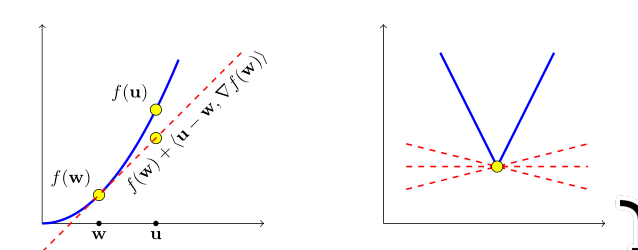
\includegraphics[width=0.8\textwidth]{figures/SubGradient.png}
  \end{itemize}
  
\end{frame}


\begin{frame}{Example Generalized Online Gradient Descent}
  Consider the $\ell_2$ setup where the functions $f_1,f_2,\ldots$ are convex (but not necessarily differentiable).
  Let $\eta$ be the learning rate.
\[
  \mathred{w_{t+1} = w_t - \eta z_t,\;\;
    z_t \in \partial f_t(w_t)}
\]
Identical to FTRL with regularization: $\mathred{R(w) = \frac{1}{2\eta}\|w\|_2^2}$

{\bf Regret bound on OGD:} From FTRL theorem:
\begin{align*}
\mathred{\text{Regret}} &\mathred{\leq \frac{\|u\|^2}{2\eta} + \eta \sum_{t=1}^T \|z_t\|^2} \\
&\mathred{\leq \frac{B^2}{2\eta} + \eta T L^2}
\end{align*}
\end{frame}


\begin{frame}{Online Mirror Descent (OMD)}
\textbf{parameter:} a link function \( g : \mathbb{R}^d \to S \)

\textbf{initialize:} \( \textcolor{mathcolor}{\theta_1 = 0} \)

\textbf{for} \( t = 1,2,\dots \)
\begin{itemize}
    \item \textbf{predict} \( \mathbf{w}_t = \textcolor{mathcolor}{ g(\theta_t) } \)
    \item \textbf{update} \( \theta_{t+1} = \textcolor{mathcolor}{ \theta_t - \mathbf{z}_t } \) where \( \mathbf{z}_t \in \textcolor{mathcolor}{ \partial f_t(\mathbf{w}_t) } \)
\end{itemize}
\end{frame}




\section{Duality}

\begin{frame}
  \frametitle{Duality}
  \begin{itemize}
  \item OMD can be analyzed using elementary tools.
    \item Using Duality Gives better intuition, more general analysis, tighter bounds.
  \end{itemize}
\end{frame}

\begin{frame}
\frametitle{Dual Vector Spaces}

\begin{itemize}
\item \R{$V$} is a vector space, with a norm \R{$\|v\|$}
\item \R{$U$} is the set of all linear mappings from \R{$V$} to
  \R{$V$}
  \item
  The norm of \R{$u \in U$} is defined as
  \R{$$\|u\|^* = \max_{v \in V} \frac{\|u(v)\|}{\|v\|}$$}
\item \R{$V$} is equivalent to the set of all linear mappings from \R{$U$} to
  \R{$U$}.
\item \R{$U$} and \R{$V$} are dual vector spaces, with dual norms. 
\end{itemize}
\end{frame}

\begin{frame}
\frametitle{Dual Norms}
\begin{itemize}
  \item The space is always \R{$U,V = \real^n$}
  \item The linear operation is the dot product \R{$\vu \cdot \vv$}
\item \R{$L_2$} norm: \R{$\sqrt{\sum_{i=1}^n x_i^2}$}
\item \R{$L_1$} norm: \R{$\sum_{i=1}^n |x_i|$}
\item \R{$L_\infty$} norm: \R{$\max_i |x_i|$}
\item \R{$L_p$} norm: \R{$\paren{\sum_{i=1}^n x_i^p}^{\frac{1}{p}}$}
\item \R{$L_p,L_q$} are dual norms if \R{$p,q \geq 1, \mbox{ and }\frac{1}{p} + \frac{1}{q} = 1$}
\item \R{$L_1,L_\infty$} are dual.
\item \R{$L_2$} is self-dual. 
\end{itemize}
\end{frame}

\begin{frame}
\frametitle{Fenchel Duality}
\begin{itemize}
\item Suppose \R{$F:A \to \real$} is a convex function over a convex set \R{$A
    \subseteq \real^n$}.
\item The dual function to \R{$F$} is
  \R{$$
    F^*(\vu) = \sup_{\vv \in A}\paren{\vu \cdot \vv -F(\vv)}
$$}
  \item Fenchel duality Reduces to Legendre duality for differentiable functions

\end{itemize}
\end{frame}

\begin{frame}
  \frametitle{Visualization of the Febchel Dual}
  \begin{columns}
    \begin{column}{0.55\textwidth}
        \begin{itemize}
            \item \R{$x,y \real$}
            \item \R{$ f^*(y) = \sup_{x \in \real}\paren{xy-f(x)}$}
            \item \R{$ -f^*(y) = \inf_{x \in \real}\paren{f(x)-xy}$}
        \end{itemize}
    \end{column}
    \begin{column}{0.43\textwidth}
          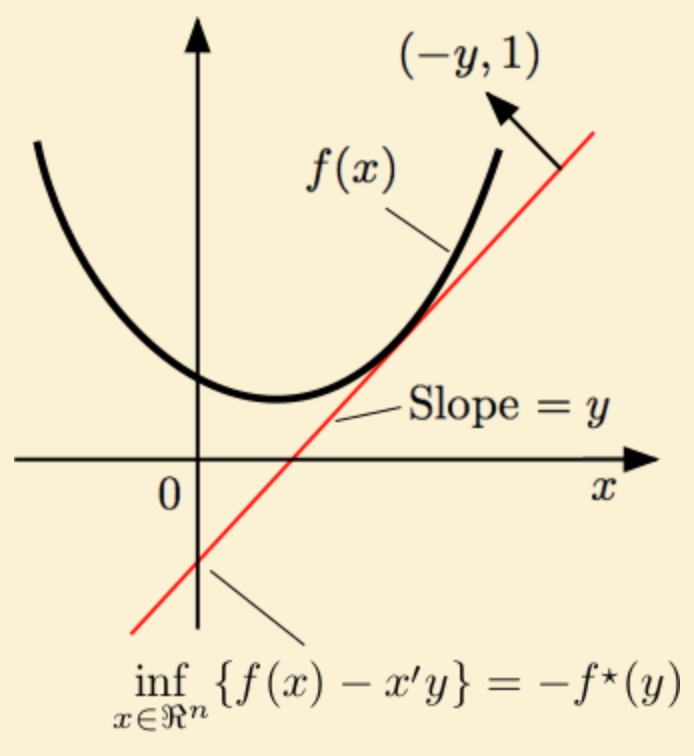
\includegraphics[width=\textwidth]{figures/Legendre-Duality.png}
    \end{column}
\end{columns}
\end{frame}

\begin{frame}
  \frametitle{Dual of Dual}
  \begin{itemize}
  \item The dual of any function is convex.
  \item if \R{$F$} is convex then \R{$F^{**} = F$}
  \end{itemize}
  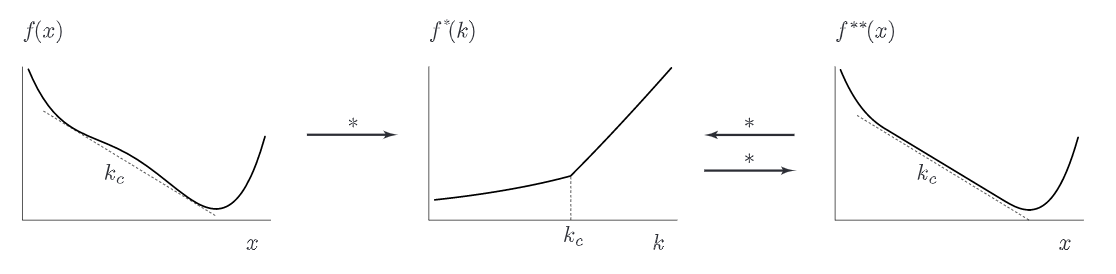
\includegraphics[width=\textwidth]{figures/FromNonConvexToConvex.png}  
\end{frame}

\begin{frame}
  \frametitle{Gradient Duality}
  \begin{itemize}
  \item
    If the gradient of \R{$f$} at \R{$x$} is \R{$k$} then\\
    the gradient of \R{$f^*$} at \R{$k$} is \R{$x$}
    \item In general:
  \R{$$
    \nabla F^* = \paren{\nabla F}^{-1}
    $$}
  \end{itemize}
  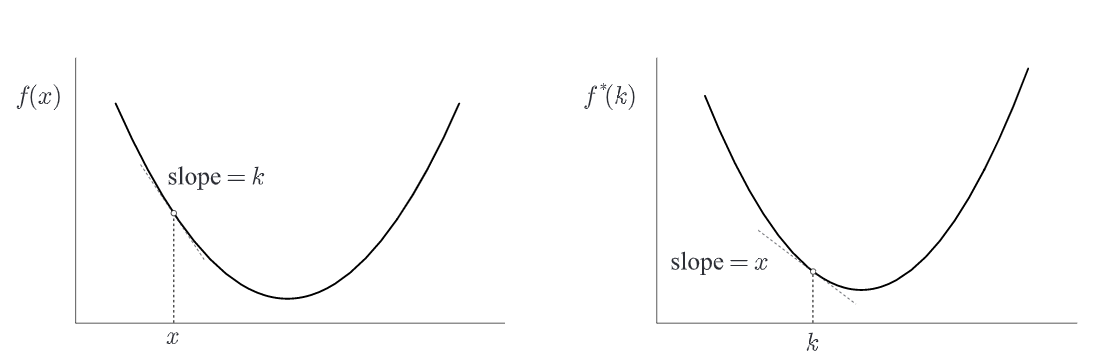
\includegraphics[width=\textwidth]{figures/SlopeDuality.png}
\end{frame}

\begin{frame}
  \frametitle{Example: Exponential Potential}
  \begin{itemize}
  \item Potential: \R{$F(\vu) = \sum_{i=1}^d e^{u_i}$}
  \item Gradient: \R{$\nabla F(\vu)_i = e^{u_i}$} or \R{$\nabla F(\vu)
      = F(\vu)$}.
  \item Dual:  \R{$F^*(\vv) = \sum_{i=1}^d v_i (\ln v_i -1)$}
  \item Gradient of dual: \R{$\nabla F^*(\vv)_i = \ln v_i $} 
  \item Note \R{$(\nabla F)^{-1} = \nabla F^*$}
   \end{itemize}
 \end{frame}

 \begin{frame}
    \frametitle{Bregman Divergence}
   \begin{columns}
     \begin{column}{0.55\textwidth}
       \begin{itemize}
       \item \R{$R(x)$} is convex and differentiable.
       \item \R{$D_R(w||u) = R(w)-(R(u) + \langle \nabla R(u) , (w-u) \rangle)$}
       \end{itemize}
     \end{column}
      \begin{column}{0.43\textwidth}
        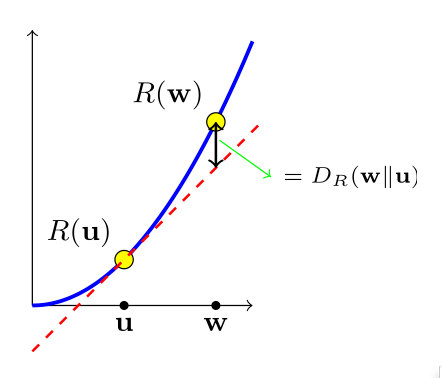
\includegraphics[width=\textwidth]{figures/BregmanDivergence.png}
      \end{column}
    \end{columns}
  \end{frame}
 
\begin{frame}
  \frametitle{Fenchel and Bregman}
  \begin{itemize}
  \item
    \R{$F$}: strictly convex with continuous first derivative.
  \item \R{$F^*$} is the Fenchel Dual of \R{$F$}
  \item \R{$D_F,D_{F^*}$} Bregman divergences wrt \R{$F,F^*$}
  \item \R{$\vu' = \nabla F(\vu)$} and \R{$\vv' = \nabla F(\vv)$}
  \item \R{$D_F(\vu,\vv)  = D_{F^*}(\vu',\vv')$}
  \end{itemize}
\end{frame}

\begin{frame}
  \frametitle{Mirror Descent}
  \begin{itemize}
  \item Gradient descent in dual space
    \R{$\theta_t = \theta_{t-1} - \lambda \nabla \ell_t(\theta_{t-1})$}
  \item Using duality can be rewritten as
    \R{$$\nabla \Phi^*(\vw_t) =  \nabla \Phi^*(\vw_{t-1})  - \lambda \nabla \ell_t(\vw_{t-1})$$}
  \item As \R{$\nabla \Phi$} is the inverse of \R{$\nabla \Phi^*$} we get
    \R{$$ \vw_t = \nabla \Phi \paren{\nabla \Phi^*(\vw_{t-1})  - \lambda \nabla \ell_t(\vw_{t-1})}$$}
  \end{itemize}
\end{frame}

\begin{frame}
  \frametitle{A picture of mirror descent}
\R{$$ \vw_t = \nabla \Phi \paren{\nabla \Phi^*(\vw_{t-1})  - \lambda \nabla \ell_t(\vw_{t-1})}$$}
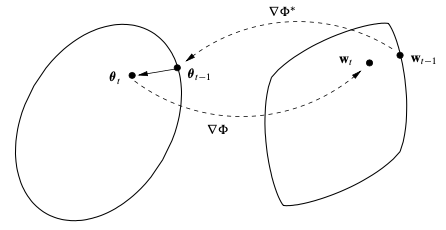
\includegraphics[width=\textwidth]{figures/MirrorDescent.png}
\end{frame}

%%%%%

\begin{frame}{Mirror Descent Regret Bound}
\textbf{Goal:} Minimize regret in online convex optimization:

\[
\text{Regret}(T) = \sum_{t=1}^{T} \langle w_t - w^*, z_t \rangle.
\]

\textbf{Mirror Descent Update Rule:}
\[
w_{t+1} = \arg\min_{w \in \mathcal{W}} \left[ \eta \langle w, z_t \rangle + D_R(w \| w_t) \right].
\]

where:
\begin{itemize}
    \item \( R(w) \) is a \textcolor{mathcolor}{strongly convex} potential function.
    \item \( D_R(w \| u) \) is the \textcolor{mathcolor}{Bregman divergence}:
    \[
    D_R(w \| u) = R(w) - R(u) - \langle \nabla R(u), w - u \rangle.
    \]
\end{itemize}
\end{frame}

\begin{frame}{Step 1: Understanding the First-Order Optimality Condition}
\textbf{Why does the first-order optimality condition hold?}

Since \( w_{t+1} \) minimizes the mirror descent objective:

\[
w_{t+1} = \arg\min_{w} \left[ \eta \langle w, z_t \rangle + D_R(w \| w_t) \right],
\]

the function being minimized is **convex**. Hence, its **first-order optimality condition** states:

\[
\langle w - w_{t+1}, \eta z_t + \nabla R(w_{t+1}) - \nabla R(w_t) \rangle \geq 0, \quad \forall w.
\]

\textbf{Interpretation:} This inequality means that at \( w_{t+1} \), the directional derivative of the objective function is **non-negative** for all feasible points, ensuring that \( w_{t+1} \) is a minimizer.
\end{frame}

\begin{frame}{Step 2: Applying the Optimality Condition to Regret}
Setting \( w = w^* \) in the optimality condition:

\[
\langle w^* - w_{t+1}, \eta z_t + \nabla R(w_{t+1}) - \nabla R(w_t) \rangle \geq 0.
\]

Rearrange:

\[
\langle w^* - w_{t+1}, \eta z_t \rangle \geq \langle w^* - w_{t+1}, \nabla R(w_{t+1}) - \nabla R(w_t) \rangle.
\]

\textbf{Key Idea:} The **gradient of \( R \) acts as a mirror map**, ensuring that updates remain in the feasible region.
\end{frame}

\begin{frame}{Step 3: Using the Three-Point Bregman Identity}
\textbf{Bregman divergence identity:}

\[
D_R(w^* \| w_t) - D_R(w^* \| w_{t+1}) - D_R(w_{t+1} \| w_t) = \langle w^* - w_{t+1}, \nabla R(w_{t+1}) - \nabla R(w_t) \rangle.
\]

Substituting into our previous inequality:

\[
\langle w^* - w_{t+1}, \eta z_t \rangle \geq D_R(w^* \| w_t) - D_R(w^* \| w_{t+1}) - D_R(w_{t+1} \| w_t).
\]

Rearrange:

\[
\langle w_t - w^*, z_t \rangle \leq \frac{1}{\eta} \left(D_R(w^* \| w_t) - D_R(w^* \| w_{t+1}) \right).
\]
\end{frame}

\begin{frame}{Step 4: Summing Over All Iterations}
Summing from \( t = 1 \) to \( T \):

\[
\sum_{t=1}^{T} \langle w_t - w^*, z_t \rangle \leq \frac{1}{\eta} \sum_{t=1}^{T} \left(D_R(w^* \| w_t) - D_R(w^* \| w_{t+1}) \right).
\]

\textbf{Why does this work?}
\begin{itemize}
    \item The sum on the right forms a **telescoping series**.
    \item All intermediate terms cancel, leaving:
\end{itemize}

\[
\sum_{t=1}^{T} \langle w_t - w^*, z_t \rangle \leq \frac{1}{\eta} (D_R(w^* \| w_1) - D_R(w^* \| w_{T+1})).
\]

\textbf{Since Bregman divergence is non-negative:}

\[
\sum_{t=1}^{T} \langle w_t - w^*, z_t \rangle \leq \frac{1}{\eta} D_R(w^* \| w_1).
\]
\end{frame}

\begin{frame}{Final Regret Bound}
\textbf{Conclusion: Mirror Descent Regret Bound}

\[
\sum_{t=1}^{T} \langle w_t - w^*, z_t \rangle \leq \frac{1}{\eta} D_R(w^* \| w_1).
\]

\textbf{Key Takeaways:}
\begin{itemize}
    \item **Mirror Descent minimizes cumulative loss** via \textcolor{mathcolor}{regularized updates}.
    \item The \textcolor{mathcolor}{Bregman divergence} controls how much each step deviates.
    \item The regret bound depends on the choice of **regularizer \( R(w) \)**.
\end{itemize}

\textbf{Implication:} Choosing an appropriate \( R(w) \) determines the efficiency of the algorithm.
\end{frame}

%%%%%
\section{Algorithms for specific potentials}

\begin{frame}
  \frametitle{Polynomial Potential}
  \begin{itemize}
  \item Potential: \R{$\Phi_p(\vu) = \frac{1}{2} \|\vu\|_p^2= \frac{1}{2} \paren{\sum_{i=1}^d
        u_i^p}^{2/p}$}
  \item Dual Potential \R{$\Phi_p^* = \Phi_q$} Where
    \R{$\frac{1}{p}+\frac{1}{q} = 1$}
  \item Euclidean norm: \R{$q=p=2$}
  \item Suppose the sequence of examples
    \R{$(\vx_1,y_1),\ldots,(\vx_T,y_T)$} satisfies \R{$\| \vx_t \|_p
      \leq X_p$} for all \R{$1 \leq t \leq T$}
  \item Suppose we use the dual descend algorithm for the potential
    function \R{$\Phi_p$} and the learning rate \R{$\lambda =
      \frac{2 \epsilon}{(p-1) X_p^2}$} for some \R{$0<\epsilon<1$}
  \item \B{Loss Bound}:\\
    \R{$L_{A,T}  \leq \frac{L_T(\vu)}{1-\epsilon} + \frac{\| \vu
        \|_q^2}{\epsilon (1-\epsilon)}\times \frac{(p-1)X_p^2}{4}$}
  \end{itemize}
\end{frame}

\begin{frame}
\frametitle{Exponential Potential}
  \begin{itemize}
  \item Potential: \R{$\Phi(\vu) = \sum_{i=1}^d e^{u_i}$}
  \item Dual Potential \R{$\Phi^*(\vu) = \sum_{i=1}^d u_i (\ln u_i -1)$}
  \item Euclidean norm: \R{$q=p=2$}
  \item Suppose the sequence of examples
    \R{$(\vx_1,y_1),\ldots,(\vx_T,y_T)$} satisfies \R{$\| \vx_t \|_\infty
      \leq X_p$} for all \R{$1 \leq t \leq T$}
  \item Suppose we use the dual descend algorithm for the exponential potential
    function \R{$\Phi$} and the learning rate \R{$\lambda =
      \frac{2 \epsilon}{X_{\infty}^2}$}  for some \R{$0<\epsilon<1$}
  \item \B{Loss Bound}:\\
    \R{$L_{A,T}  \leq \frac{L_T(\vu)}{1-\epsilon} + \frac{X_\infty^2
        \ln d}{2 \epsilon (1-\epsilon)}$}
  \end{itemize}
\end{frame}

\begin{frame}{Lemma 2.20: Regret Bound for OMD}
\textbf{Lemma 2.20.} Suppose that OMD is run with a link function \( g = \nabla R^* \). Then, its regret is upper bounded by:

\[
\sum_{t=1}^{T} \textcolor{mathcolor}{ \langle \mathbf{w}_t - \mathbf{u}, \mathbf{z}_t \rangle }
\leq \textcolor{mathcolor}{ R(\mathbf{u}) - R(\mathbf{w}_1) }
+ \sum_{t=1}^{T} \textcolor{mathcolor}{ D_{R^*}(-\mathbf{z}_{1:t} \| -\mathbf{z}_{1:t-1}) }.
\]

Furthermore, equality holds for the vector \( \mathbf{u} \) that minimizes \( \textcolor{mathcolor}{ R(\mathbf{u}) + \sum_t \langle \mathbf{u}, \mathbf{z}_t \rangle } \).
\end{frame}

\end{small}
\end{document}
%%%%%%%%%%%%%%%%%%%%%%%%%%%%%%%%%%%%
\begin{frame}
\begin{proof}
Using lemma 3.3 and strong convexity:
\begin{align*}
\mathred{\sum_{t=1}^T \langle w_t - u, z_t \rangle} &\mathred{\leq \frac{1}{2\eta}\|u\|^2 + \eta \sum_{t=1}^T \|z_t\|^2} \\
&\mathred{\leq \frac{B^2}{2\eta} + \eta T L^2}
\end{align*}
Minimizing over $\mathred{\eta}$ gives $\mathred{O(\sqrt{T})}$ bound
\end{proof}
\end{frame}


%%% Local Variables:
%%% mode: latex
%%% TeX-master: t
%%% End:
